%%%  default
\documentclass[10pt, compress, aspectratio=43]{beamer}


\usetheme{mnuigD}
\usepackage{tikz}
\usepackage{booktabs}
%\usepackage{cite}
\usepackage{hyperref}
\bibliographystyle{apalike}
\usepackage[export]{adjustbox}
\usepackage{subfig}
\usepackage[export]{adjustbox}
% \usepackage[scale=2]{ccicons}
\usepackage[normalem]{ulem} % for strikethorugh
%\usemintedstyle{trac}
\usepackage{grffile} %for underscores in file names
\title{Software Carpentry: \\Teaching basic lab skills for research computing}
\subtitle{{\small (or, an investment in tomorrow's sanity)}}
% \subtitle{NUIG Bioinformatics}
\date{\footnotesize{ \today}}
\author{
  % \vspace{10mm}
  % \hspace{5mm}
\includegraphics[height=30mm]{./20170202_bss_figs/logo_1_dark}
\\ \\ \\ \\ \large{Nick Waters}}
\institute{}
% National University of Ireland, Galway\\
% James Hutton Institute, Dundee}

%%%%% %%%%% %%%%% %%% %%%%  for pretty headers with pictures
%%%%%%%%
\usepackage{xcolor}
\newcommand\ytl[2]{
\parbox[b]{8em}{\hfill{\color{cyan}\bfseries\sffamily #1}~$\cdots\cdots$~}\makebox[0pt][c]{$\bullet$}\vrule\quad \parbox[c]{4.5cm}{\vspace{7pt}\color{red!40!black!30}\raggedright\sffamily #2\\[7pt]}\\[-3pt]}


%%%%%%%%%%%%%%%%%%%%%%%%%%%%%%%%%%%%%%

\begin{document}
\maketitle

%\maketitle
\setbeamertemplate{itemize items}[square]

\begin{frame}[fragile]
  \frametitle{How can scientific programming help your work?}

  \begin{itemize}[<+- | alert@+>]
  \item automation $\rightarrow$ reproducibility
  \item Do more in less time (BLAST, CLUSTAL, etc.)
  % \item Use cutting-edge analysis software
  \item Automate repetitive tasks
  \item Analyze NGS data
  \end{itemize}
\end{frame}


\begin{frame}
  \frametitle{attrib. Dr. Paul Ehrlich}
      \begin{columns}[onlytextwidth]
        \column{0.4\textwidth}
        \begin{itemize}
        \item<2- > \textit{To err is human, but to really foul things up you need a computer.}
        \end{itemize}
        \column{0.1\textwidth}
        \column{0.5\textwidth}
        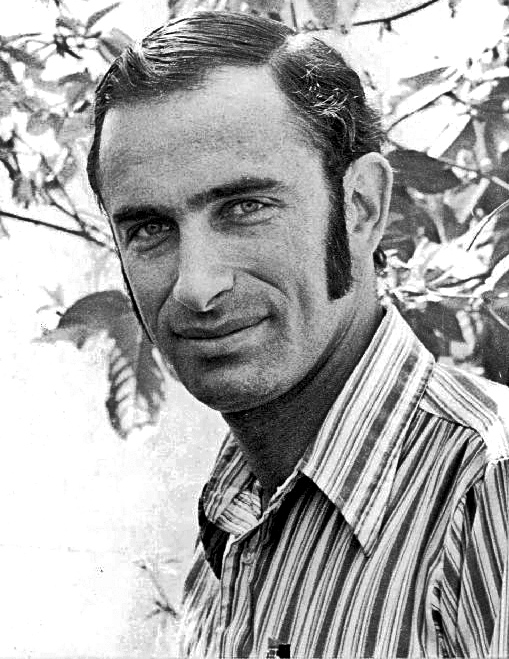
\includegraphics[height=4cm]{./frequentFigs/Paul_Ehrlich.jpg}
        \end{columns}
  \end{frame}


\begin{frame}[fragile]
  \frametitle{Results of lack of training}
  \begin{itemize}[<+- | alert@+>]
  \item Getting tricked by software
  \item Missing or unusable electronic lab notebooks
  \end{itemize}
\end{frame}

\begin{frame}{What is Software Carpentry?}
  \href{https://software-carpentry.org/workshops/pitch/}{
\includegraphics[height=1cm]{./frequentFigs/swc.png}}% [1]

  Since 1998, Software Carpentry has been teaching researchers the computing skills they need to get more done in less time and with less pain
\visible<2- >{
  \begin{table}
  % \caption{Timeline of something.}
    \centering
    \begin{minipage}[t]{.7\linewidth}
      \color{gray}
      \rule{\linewidth}{1pt}
      \ytl{Shell}{Automating tasks, connecting to clusters, transferring data}
      \ytl{Git}{Tracking version history}
      \ytl{R/Python}{Writing resuable, reliable software }
      \rule{\linewidth}{1pt}%
    \end{minipage}%
  \end{table}
}
\end{frame}

\begin{frame}{Bringing SWC to NUIG}
  Cost: €500 fee + travel and expenses for instructor, and catering\\
  \vspace{.5cm}
  \visible<2- >{How can you help?}
  \visible<3- >{\begin{itemize}%[<+- | alert@+>]
  \item Encourage lab members to attend
  \item Help cover cost of instructor travel
  \end{itemize}}
\end{frame}



\begin{frame}{Benefits }
  \begin{itemize}
            % \alert<2>{\only<2>{\LARGE \textbf{Questions?}}}
  \visible<2- >{\item \textit{Average time saved: $\frac{1}{2}$ to 1 day \textbf{per week}}}
  \end{itemize}
  \vspace*{2.6cm}
    \visible<3- >{\color{yellow} \Large{questions?}}
\end{frame}


\begin{frame}{Resources}
  \begin{itemize}
  \item {\color{green} \href{https://mikecroucher.github.io/MLPM_talk/}{Is your Research Sofware Correct?}}
    \item {\color{green}\href{https://genomebiology.biomedcentral.com/articles/10.1186/s13059-016-1044-7}{Zeimann et al's Excel gene name paper}}
  \end{itemize}
\end{frame}




\end{document}
